\documentclass[tikz, border=2mm]{standalone}
\usepackage{tikz}
\usepackage{amsmath,amssymb}
\usepackage[]{xcolor}
\usepackage{graphicx}
\usepackage{tikz-3dplot}
\usetikzlibrary{arrows.meta, decorations.pathmorphing}

\begin{document}

\def\xoffset{0.2}
\def\yoffset{0.0}
\def\zoffset{0.5}
\def\viewphi{135}
\def\viewtheta{60}
\def\orthoScale{1.2000000476837158}


\tdplotsetmaincoords{\viewtheta}{\viewphi}

\def\imwidth{6}

\newcommand{\viewscope}[1]{
    \begin{scope}[tdplot_main_coords, scale = \imwidth/\orthoScale]
        % shift the origin to the desired location
        \coordinate (Shift) at (-\xoffset,-\yoffset,-\zoffset);
        \tdplotsetrotatedcoordsorigin{(Shift)}

        \begin{scope}[tdplot_rotated_coords]
            #1
        \end{scope}
    \end{scope}
}

\begin{tikzpicture}[
    point/.style={circle, fill, inner sep=1.5pt},
    pics/sample/.style={code={\draw[#1] (0,0) -- (0.3,0);}},
]

    \viewscope{
        % a simple coordinate frame
            \draw[-latex, very thick, red] (0,0,0) -- (0.5,0,0) node[anchor=north east]{$x$};
            \draw[-latex, very thick, green] (0,0,0) -- (0,0.5,0) node[anchor=north west]{$y$};
            \draw[-latex, very thick, blue] (0,0,0) -- (0,0,0.5) node[anchor=south]{$z$};
    }


        % include the robot image as a background

    \node[opacity=0.7] at (0,0) {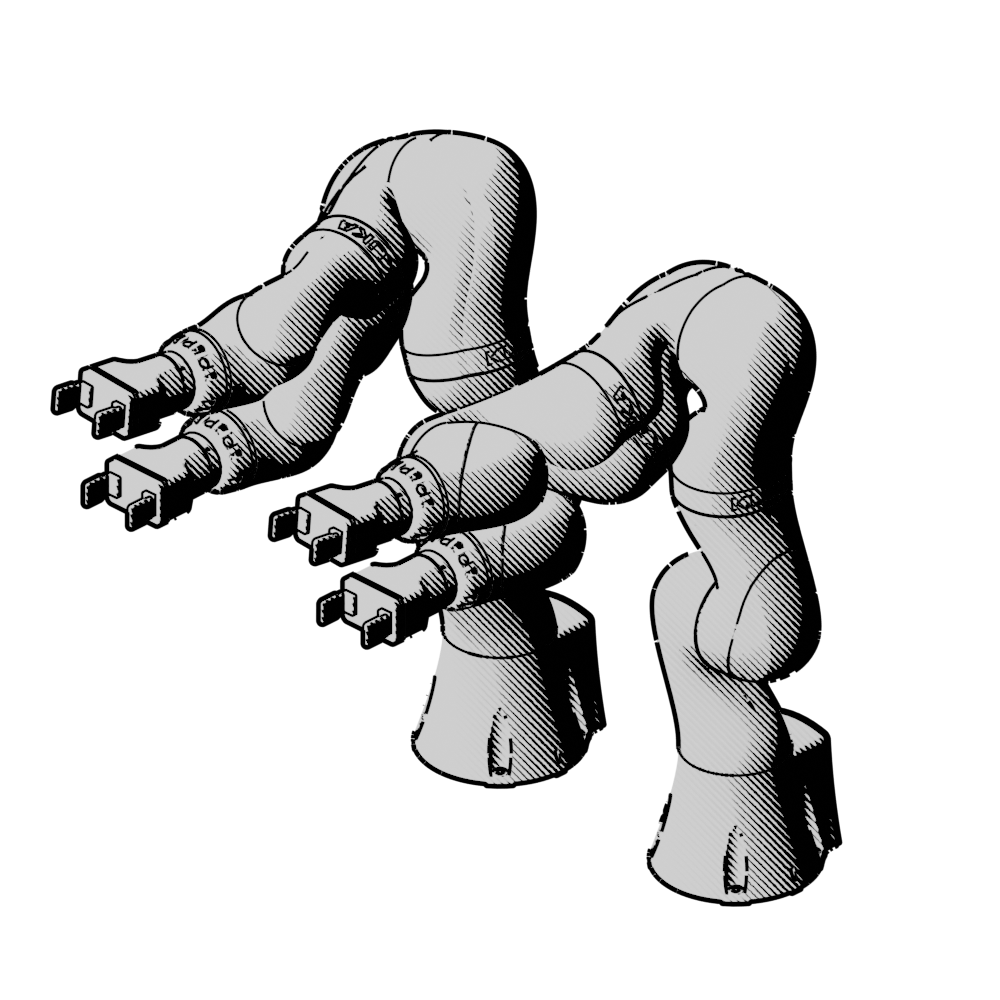
\includegraphics[width=\imwidth cm]{robot_0000_.png}};
    \node at (0,0) {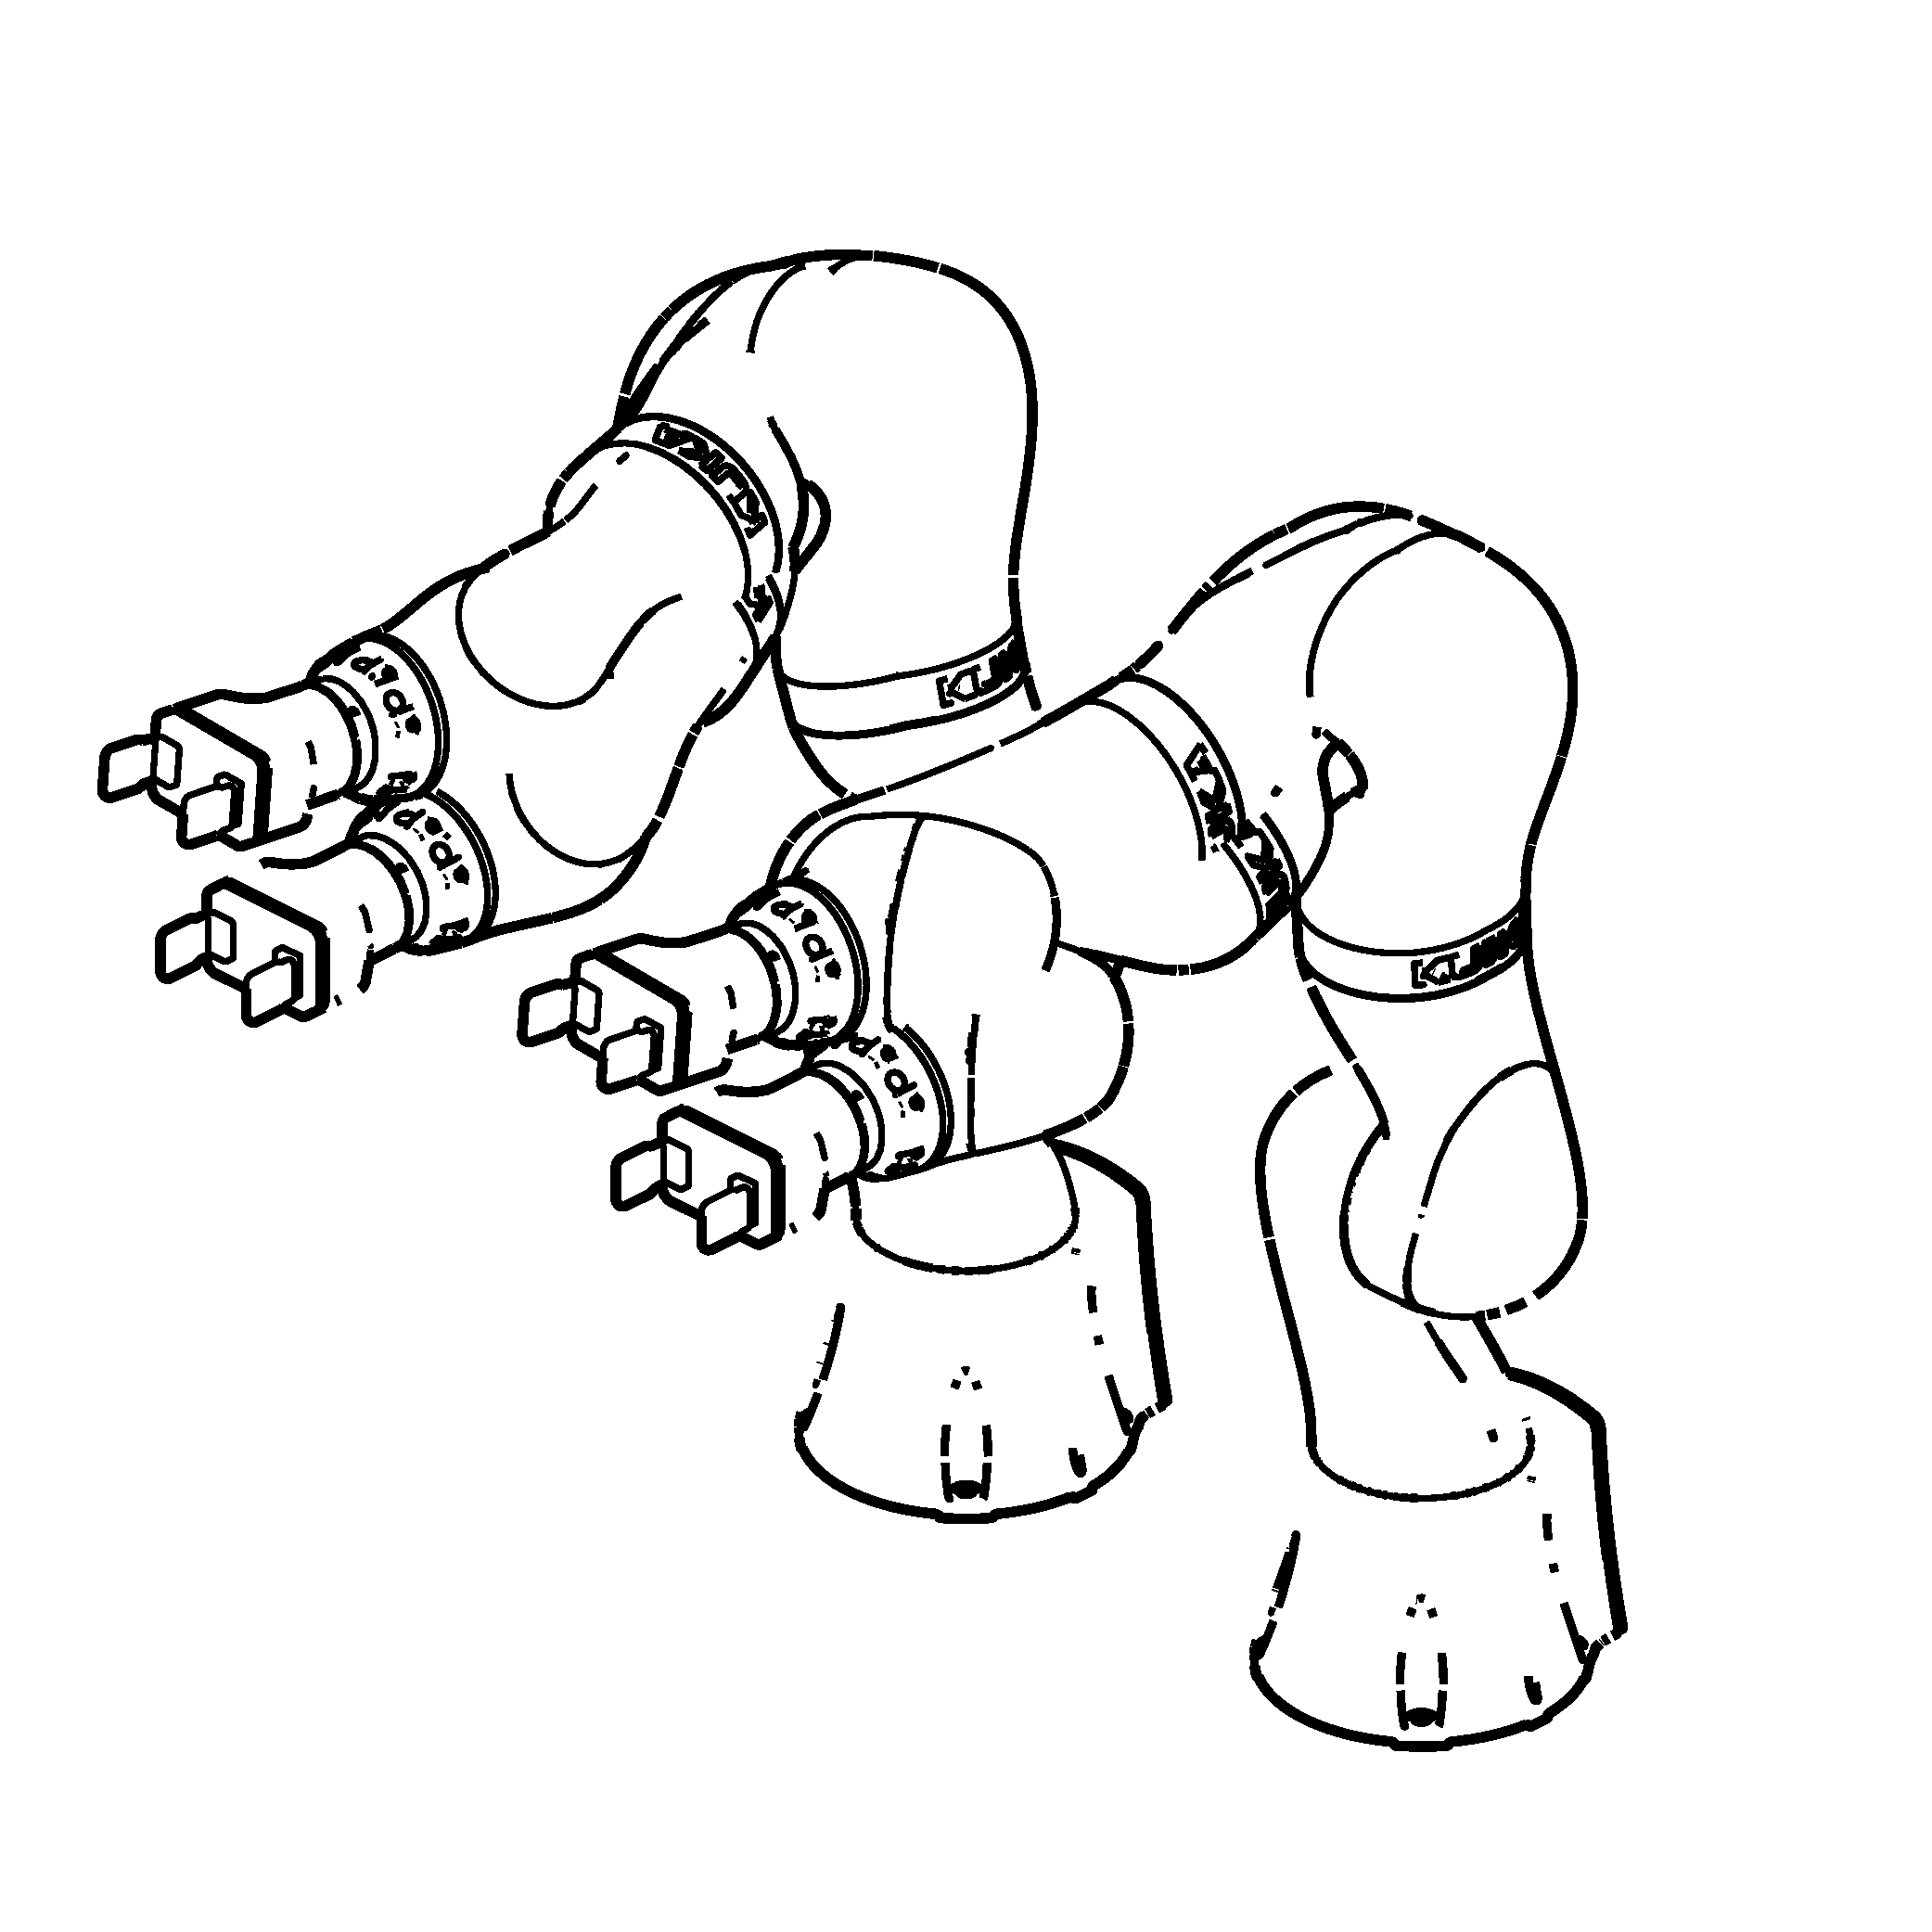
\includegraphics[width=\imwidth cm]{robot_0000_0000.pdf}};

\end{tikzpicture}
\end{document}
